\subsection{Test Configuration}

Our benchmark was tested on a 72-core (4 sockets with 18 cores each capable of running 2 hardware threads, totaling 144 hardware threads) Intel Xeon machine clocked at 2.50 GHz with 512 GB of RAM and 4 memory banks. The machine is running Ubuntu 14.04 with kernel verion 3.13.0-141. The with DEF code was compiled with DEF version 0.16.1a and the C code was compiled with Clang 6.0, and all code was compiled with -03 level of optimisation.

During the benchmark threads were pinned programmatically to inidvidual cores initially avoiding HyperThreading and later exhausting all inidivual exection units on a single CPU with the use of HyperThreading, before migrating to another CPU socket. The scalable JEMalloc\cite{JEMalloc} allocator was used in all tests, as it had been in the Forkscan paper.\cite{Forkscan} The \texttt{numactl} Linux program was used to control which memory bank allocation was allowed to take place. The memory banks closest to the running CPUs were selected as they became active.

The microbenchmark measures the number of operations carried out over a specified amount of time rather than the time taken to exectute a specified number of iterations. The rationale for this is threads finish their iterations before other threads. The remaining threads complete their iterations with less contention in the system, skewing the overall benchmark. Our benchmark reports the number of operations per second. The primary comparison is between the leaky C and the forkscan enabled DEF implementations. Each benchmark is run for a total of 20 seconds each, with each configuration being sampled 5 times. The average of the runs is plotted with error bars show the maximum variation in each run.

\subsection{Benchmark Results}

\begin{figure}[htbp!]
  \centering
  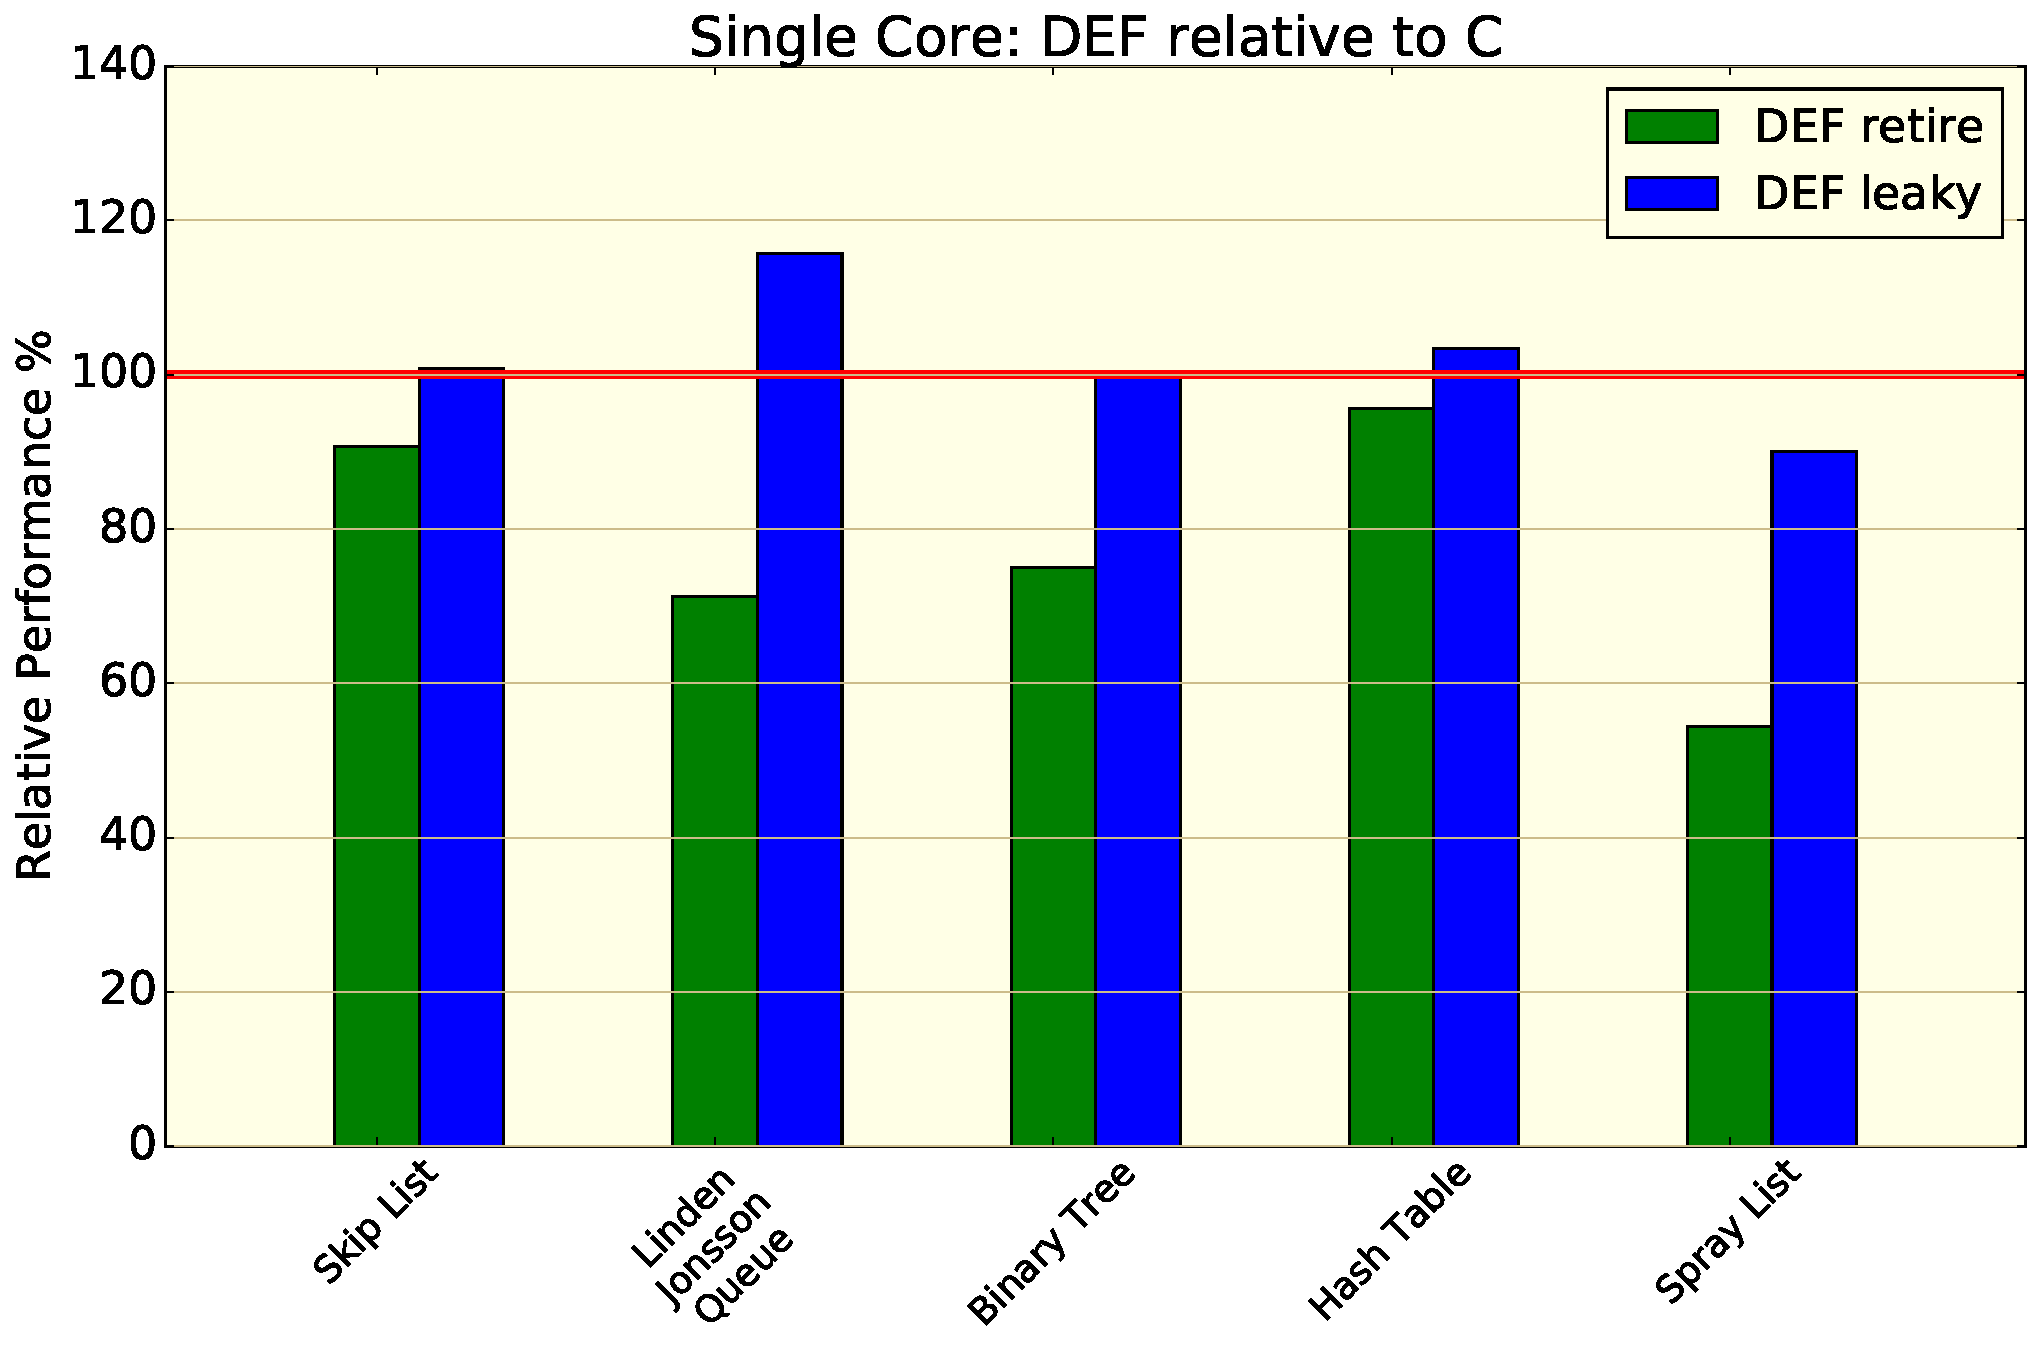
\includegraphics[scale=0.25]{gfx/RelativePerf.pdf}
  \caption{Relative performance of DEF to C on a single thread.  100\% is equivalent, and higher is better.}
  \label{fig:relativeperf}
\end{figure}

Figure \ref{fig:relativeperf} shows, for all benchmarks, single-threaded performance.  The set data structures are configured with 10\% updates, and the priority queues, naturally, are 100\% updates.  For an apples-to-apples comparison with C, a non-retiring version of the DEF code is presented.  This is a meaningful test because one expects a serial C data structure to perform better when \texttt{free} is never called than when it is, and it's no different for a concurrent data structure.  As designed, DEF is close to the machine and performs comparably in this case.  We attribute any performance distinctions to slight differences in code generation.

Minor degradation in performance is observed when memory is retired. (results?)

\begin{figure*}[tbp]
  \centering
  \raisebox{-0.5\height}{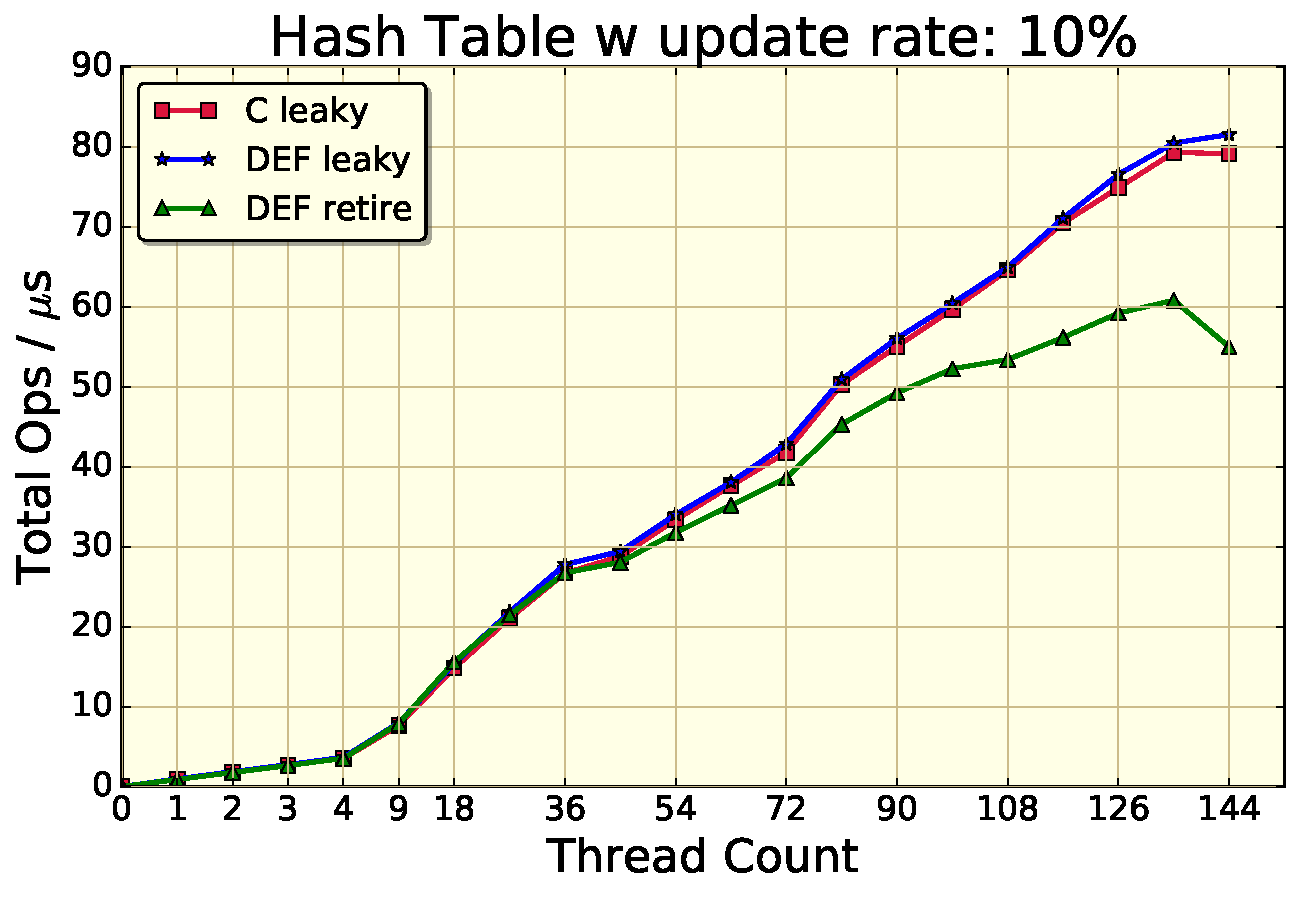
\includegraphics[scale=0.25]{gfx/HashTableLight.pdf}}
  \raisebox{-0.5\height}{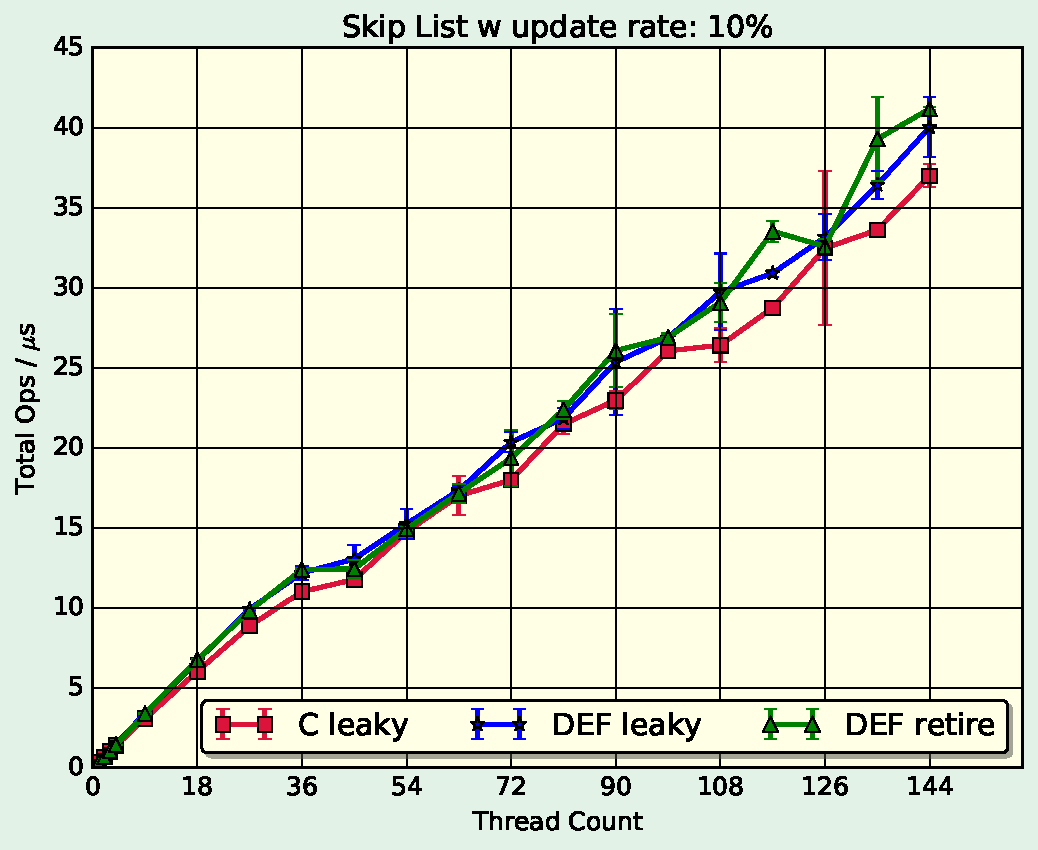
\includegraphics[scale=0.25]{gfx/SkipListLight.pdf}}
  \raisebox{-0.5\height}{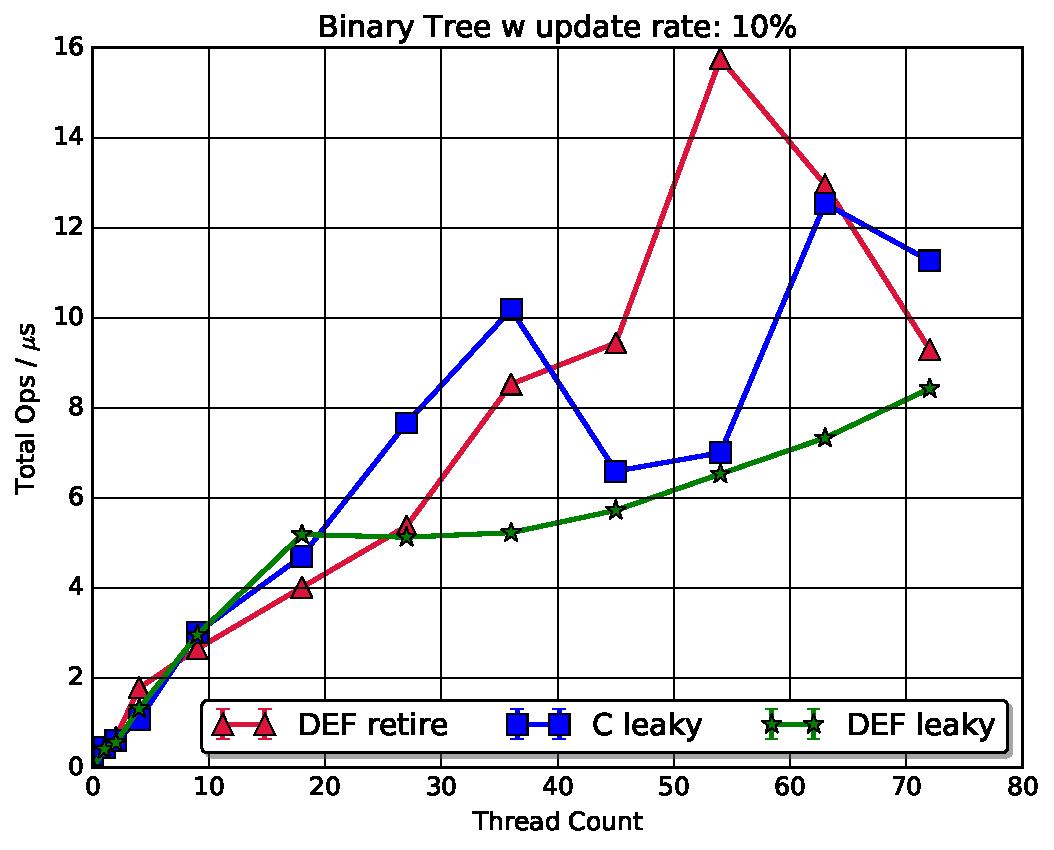
\includegraphics[scale=0.25]{gfx/BinaryTreeLight.pdf}}
  \raisebox{-0.5\height}{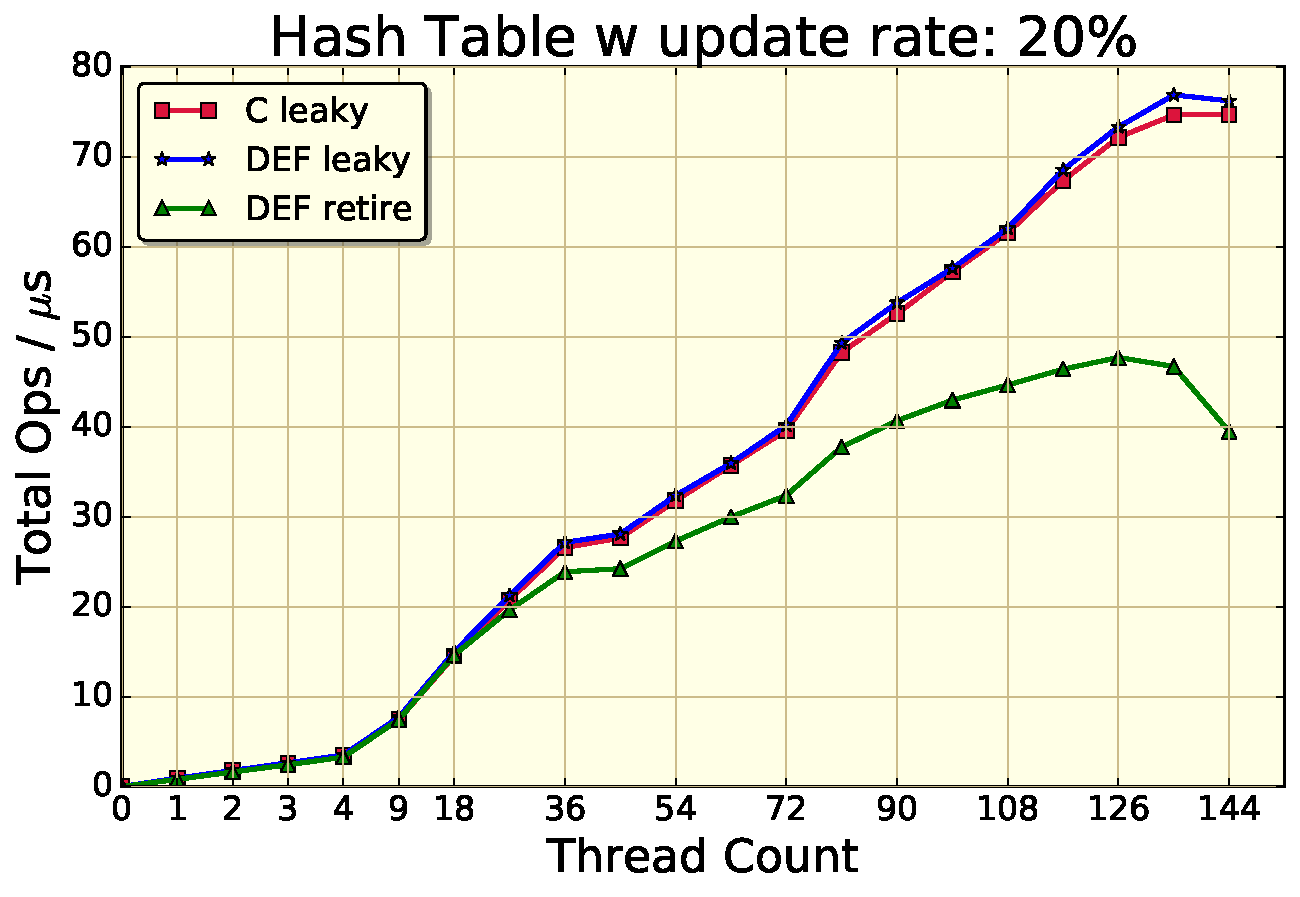
\includegraphics[scale=0.25]{gfx/HashTableMedium.pdf}}
  \raisebox{-0.5\height}{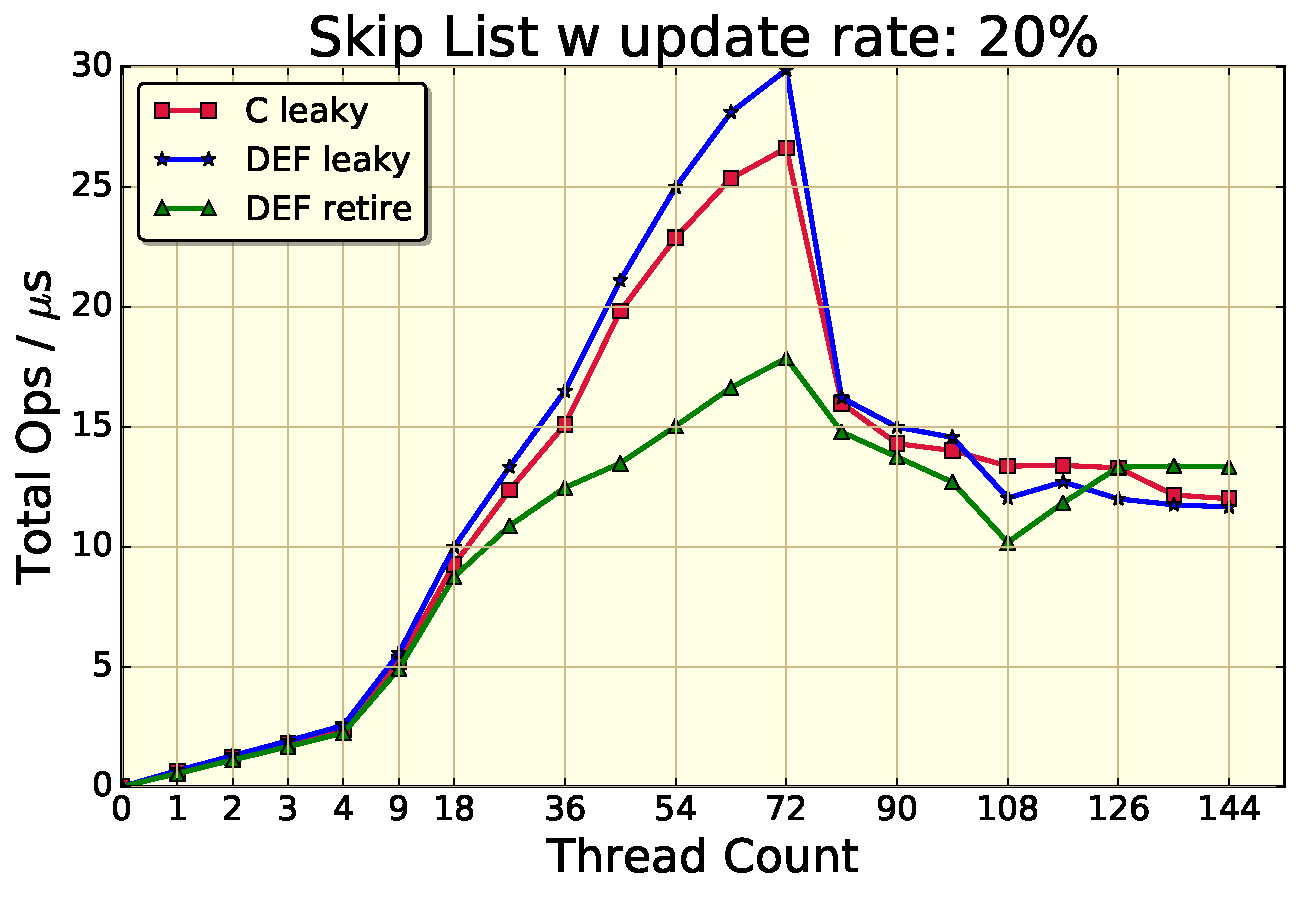
\includegraphics[scale=0.25]{gfx/SkipListMedium.pdf}}
  \raisebox{-0.5\height}{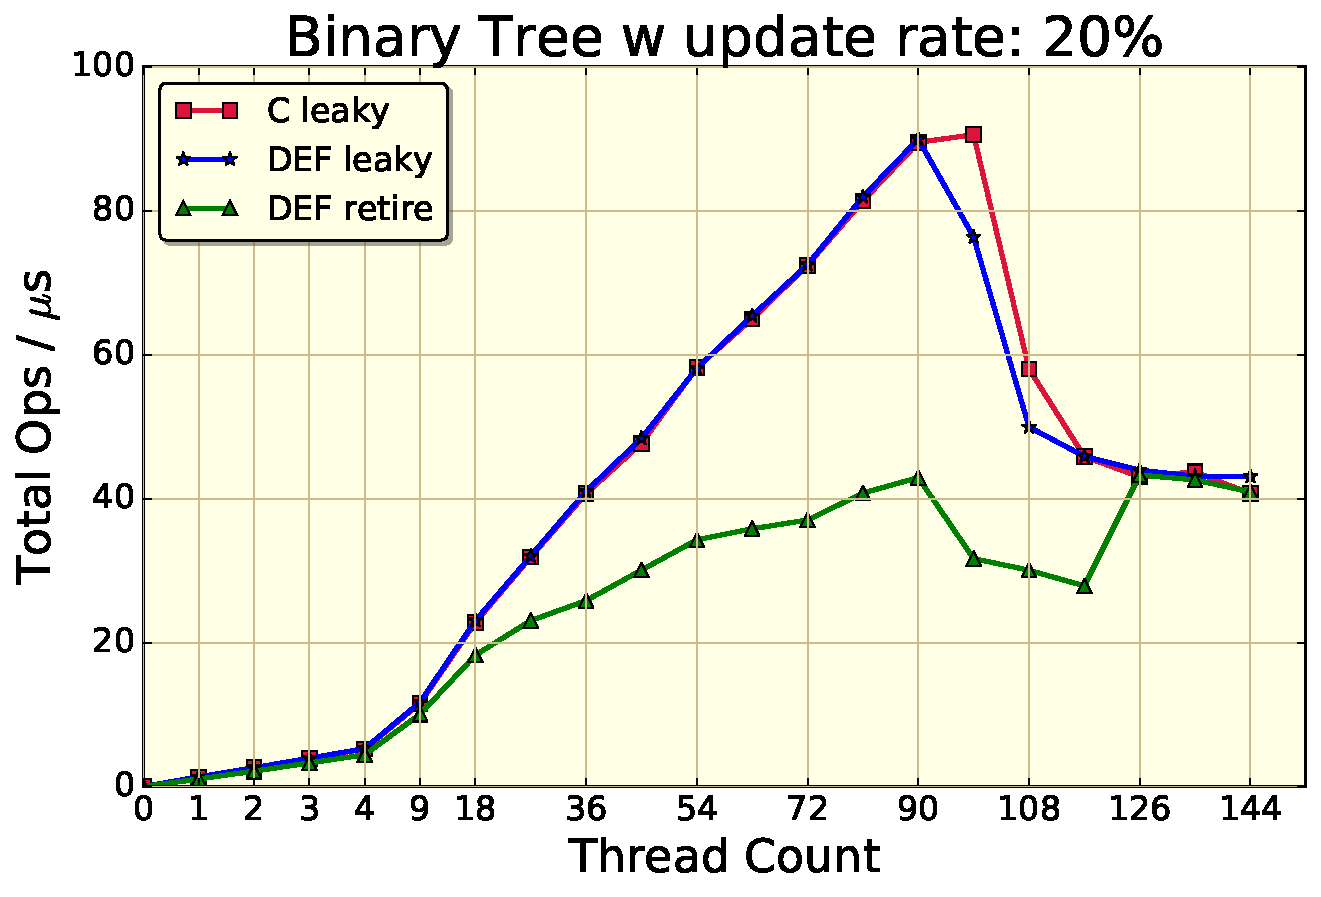
\includegraphics[scale=0.25]{gfx/BinaryTreeMedium.pdf}}
  \caption{Scalability graphs for the set data structures with 10\% (top row) and 20\% (bottom row) updates.}
  \label{fig:setdatastructures}
\end{figure*}

Scalability results for the set data structures with 10\% and 20\% updates are presented in figure \ref{fig:setdatastructures}.  As above, the three configurations were tested: Leaky-DEF, DEF, and C (also leaky).  (size of data structures in MB or GB)

C and Leaky-DEF both scale roughly linearly at 10\% updates for all three structures.  A slight hesitation is observed as they cross the NUMA boundary at 36 cores, and some affinity is visible crossing 72 threads (saturating the cores).  The non-leaky DEF versions are more gradual.  The hash table and the skip list perform with visible overhead, but consistently scale except as approaching the hyperthread limit.  This is accounted for by the fact that Forkscan creates a pool of child processes to perform the scan, up to 16, but since the application threads are pinned, the Forkscan threads get shifted around.

The binary tree tests the limits of the memory reclamation implementation, as it scales more gently and levels out around at around 90 threads.  The binary tree, similar in performance to this hash table, involves more writing per update. (is this true, Rob?)

20\% updates corresponds to an extremely write-heavy workload for real-world set data structures.  The leaky hash tables scale, but they're the most sensitive of the three structures to memory layout.  Since Leaky-DEF was slightly outperforming C, it reached the memory bandwidth limitations before C did. (verify?)  The retiring DEF code was jittery at higher thread counts for the same reason, as it ran its root-finding algorithm.

The skip list, at that rate, saturated the memory bandwidth of the machine earlier because it's more traversal-heavy than the hash table.  The larger process also made scanning take long enough that Forkscan throttled.


\begin{figure*}[tbp]
  \centering
  \raisebox{-0.5\height}{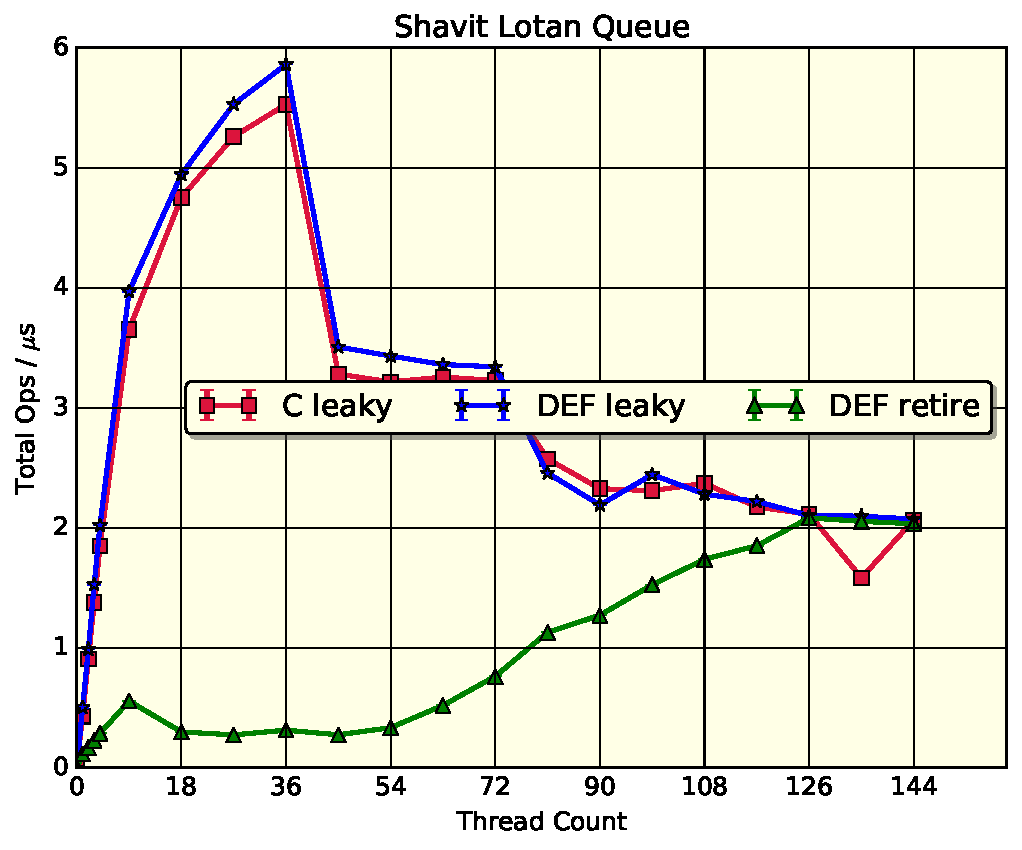
\includegraphics[scale=0.25]{gfx/ShavitLotanQueue.pdf}}
  \raisebox{-0.5\height}{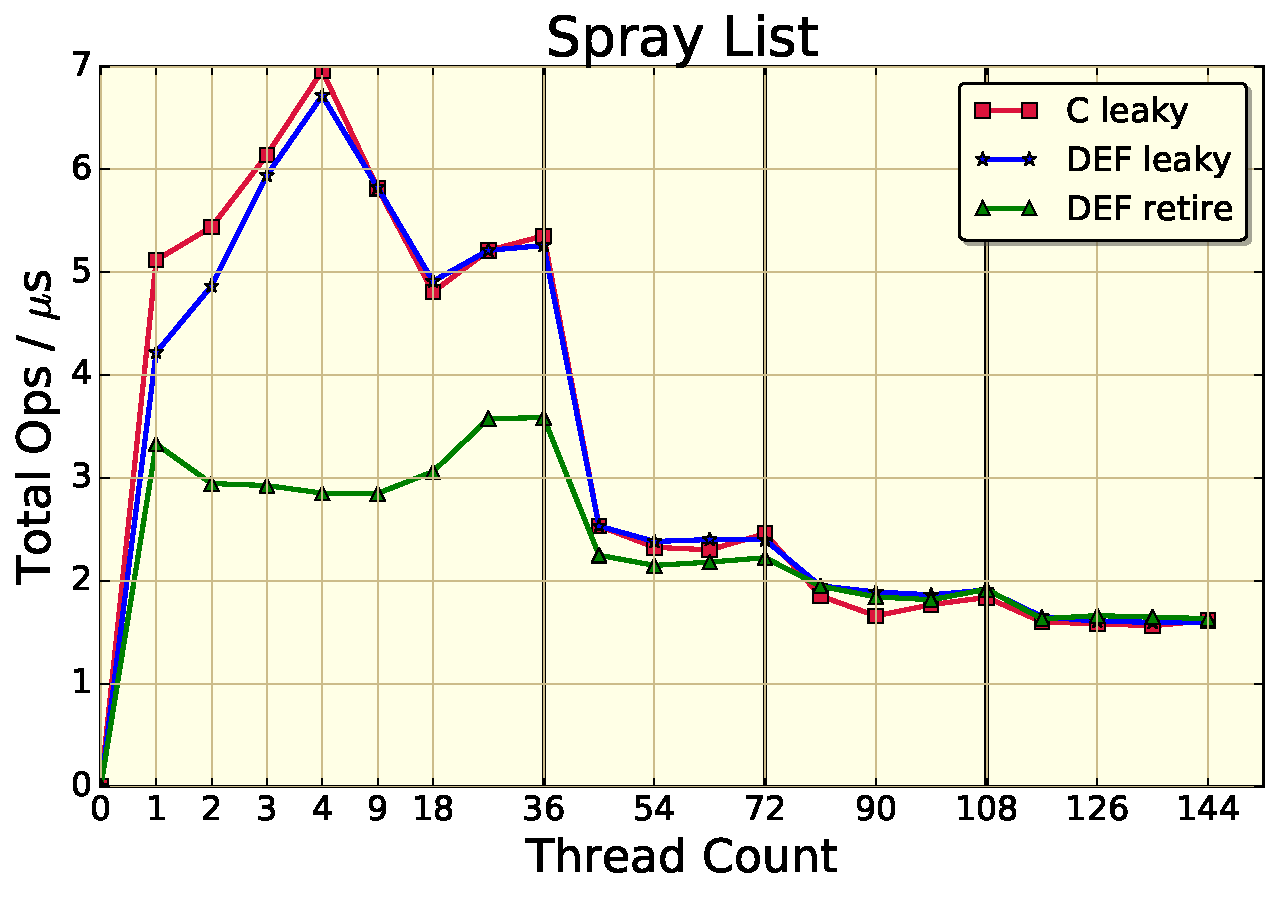
\includegraphics[scale=0.25]{gfx/SprayList.pdf}}
  \caption{Scalability graphs for the priority queues.  A priority queue's standard workload is 100\% updates.}
  \label{fig:priorityqueues}
\end{figure*}

Lastly, in figure \ref{fig:priorityqueues}, we tested the two priority queues.

